%% compile with pdflatex or xelatex
\documentclass[11pt,a4paper]{article}

\usepackage{homework}

\title{Homework 1}
\duedate{Mar 3, 2020}

\studentname{Chenhao Li}
\studentid{2017011466}

\usepackage{tikz}
\usetikzlibrary{automata,shapes,positioning,arrows}

%% logical symbols
% \land     /\
% \lor      \/
% \lnor     (negation)
% \to       ->
% \lequiv   <->
% \models   |=
\newcommand{\lequiv}{\leftrightarrow}

\begin{document}

\maketitle

\textit{Read the instructions below carefully before you start working on the assignment:}
\begin{itemize}
    \item Please typeset your answers in the attached \LaTeX~source file, compile it to a PDF,
    and finally hand the PDF to Tsinghua Web Learning \emph{before the due date}.
    \item Make sure you fill in your \emph{name} and \emph{Tsinghua ID},
    and replace all ``\texttt{TODO}''s with your solutions.
    \item Any kind of dishonesty is \emph{strictly prohibited} in the full semester.
    If you refer to any material that is not provided by us, you \emph{must cite} it.
\end{itemize}

%% problem begins

\problem{True of False}

Are the following statements true or false? If false, provide a counterexample.

\subproblem Given an arbitrary propositional logic formula, the problem of deciding its validity is decidable.

\begin{solution}
    True
\end{solution}

\subproblem If a propositional logic formula is not valid, then it is unsatisfiable.

\begin{solution}
    False
    
    Counterexample: $P$ is not valid, but it is satisfiable.
\end{solution}

\subproblem Every NNF is also a CNF.

\begin{solution}
    False
    
    Counterexample: $(P \land Q) \lor R$ is a NNF, but is not a CNF.
\end{solution}

\subproblem A propositional logic formula $\varphi$ is satisfiable if and only if for every interpretation $I$,
$I \models \varphi$.

\begin{solution}
    False
    
    $\varphi$ is satisfiable if and only if there exists interpretation $I$,
    $I \models \varphi$.
\end{solution}

\subproblem If clause $C$ is a unit under an interpretation $I$, then $I \not\models C$.

\begin{solution}
    False
    
    The value of $C$ is undefined under interpretation $I$.
\end{solution}

\newpage
\problem{Normal Forms}

\subproblem Convert the following formula into NNF and then DNF:
$$\lnot(\lnot(P \land Q) \to \lnot R)$$

\begin{solution}
	\begin{align*}
    & \lnot(\lnot(P \land Q) \to \lnot R) \\
    &= \lnot((P \land Q) \lor \lnot R) \\
    &= \lnot(P \land Q) \land R \\
    &= (\lnot P \lor \lnot Q) \land R \cdots \text{NNF} \\
    &= (\lnot P \land R) \lor (\lnot Q \land R) \cdots \text{DNF}
    \end{align*}
\end{solution}

\subproblem Convert the following formula into CNF with and without Tseitin's transformation:
$$(P \to (\lnot Q \land R)) \land (P \to \lnot Q)$$

\begin{solution}
	\begin{enumerate}
		\item With Tseitin's transformation
			\begin{align*}
			F_1 &= T_1 \lequiv \lnot Q \land R = (\lnot T_1 \lor \lnot Q) \land (\lnot T_1 \lor R) \land (T_1 \lor Q \lor \lnot R) \\
			F_2 &= T_2 \lequiv P \to T1 = (\lnot T_2 \lor \lnot P \lor T_1) \land (T_2 \lor P) \land (T_2 \lor \lnot T_1) \\
			F_3 &= T_3 \lequiv P \to \lnot Q = (\lnot T_3 \lor \lnot P \lor \lnot Q) \land (T_3 \lor P) \land (T_3 \lor Q) \\
			F_4 &= T_4 \lequiv T2 \land T3 = (\lnot T_4 \lor T_2) \land (\lnot T_4 \lor T_3) \land (T_4 \lor \lnot T_2 \lor \lnot T_3) \\
			\text{CNF} &= T_4 \land F_1 \land F_2 \land F_3 \land F_4
			\end{align*}
		\item Without Tseitin's transformation
			\begin{align*}
			& (P \to (\lnot Q \land R)) \land (P \to \lnot Q) \\
			&= (\lnot P \lor (\lnot Q \land R)) \land (\lnot P \lor \lnot Q) \\
			&= (\lnot P \lor \lnot Q) \land (\lnot P \lor R) \land (\lnot P \lor \lnot Q) \\
			\end{align*}
	\end{enumerate}
\end{solution}

\newpage
\problem{Validity \& Satisfiability}

\subproblem Consider the following formula:
$$(P \to (Q \to R)) \to (\lnot R \to (\lnot Q \to \lnot P))$$
Is it valid? If not, provide a falsifying interpretation.
Moreover, is it satisfiable? If so, provide a satisfying interpretation.

\begin{solution}
    It is not valid. There exists interpretation $I = \{P \mapsto true, Q \mapsto false, R \mapsto false \}$, such that $I \not\models F$.
    
    It is satisfiable. There exists interpretation $I = \{P \mapsto true, Q \mapsto true, R \mapsto false\}$, such that $I \models F$.
\end{solution}

\subproblem Show the validity of the following formula using the semantic argument method:
$$\lnot(P \land Q) \lequiv (\lnot P \lor \lnot Q)$$

\begin{solution}
    \begin{enumerate}
    	\item $I \not\models \lnot(P \land Q) \lequiv (\lnot P \lor \lnot Q)$
    	\item $I \models \lnot(P \land Q) \land \lnot (\lnot P \lor \lnot Q) $ (1 and $\lequiv$, case A)
    	\item $I \models \lnot(P \land Q)$ (2 and $\land$)
    	\item $I \models \lnot (\lnot P \lor \lnot Q)$ (2 and $\land$)
    	\item $I \not\models P \land Q$ (4 and $\lnot$)
    	\item $I \not\models P$ (5 and $\land$, case A)
    	\item $I \not\models \lnot P \lor \lnot Q$ (3 and $\lnot$)
    	\item $I \not\models \lnot P$ (7 and $\lor$)
    	\item $\bot$ (6 and 8)
    	\item $I \not\models Q$ (5 and $\land$, case B)
    	\item $I \not\models \lnot Q$ (7 and $\lor$)
    	\item $\bot$ (10 and 11)
    	\item $I \models (P \land Q) \land \lnot \lnot (\lnot P \lor \lnot Q) $ (1 and $\lequiv$, case B)
    	\item $I \models P \land Q$ (13 and $\land$)
    	\item $I \models P$ (14 and $\land$)
    	\item $I \models \lnot \lnot (\lnot P \lor \lnot Q)$ (13 and $\land$)
    	\item $I \not\models \lnot (\lnot P \lor \lnot Q)$ (16 and $\lnot$)
    	\item $I \models (\lnot P \lor \lnot Q)$ (17 and $\lnot$)
    	\item $I \models \lnot P$ (18 and $\lor$, case A)
    	\item $I \not\models P$ (19 and $\lnot$)
    	\item $\bot$ (15 and 21)
    	\item $I \models Q$ (14 and $\land$)
    	\item $I \models \lnot Q$ (18 and $\lor$, case B)
    	\item $I \not\models Q$ (23 and $\lnot$)
    	\item $\bot$ (22 and 24)
    \end{enumerate}

	Therefore, every branch reaches contradiction, so $F$ is valid.
\end{solution}

\subproblem Show the satisfiability of the following formula by resolution:
$$(\lnot P \lor \lnot Q) \land (\lnot P \lor R) \land (Q \lor \lnot R)$$
Then, give a general form of all satisfying interpretations.

\begin{solution}
	\begin{enumerate}
		\item $\lnot P \lor \lnot Q$
		\item $\lnot P \lor R$
		\item $Q \lor \lnot R$
		\item $\lnot P \lor \lnot R$ (1 and 3)
		\item $\lnot P \lor Q$ (2 and 3)
		\item $\lnot P$ (2 and 4)
	\end{enumerate}

	Now there is no more possible resolvent, so $F$ is satisfiable.
	
	All satisfying interpretations have the form of $\{P \mapsto false, Q, R\}$, where $Q \lor \lnot R = true$.
\end{solution}

\newpage
\problem{Modeling}

A \emph{nondeterministic finite automaton} (NFA) is given by a 5-tuple $(Q, \Sigma, \delta, I, F)$, where:
\begin{itemize}
    \item $Q$ is a finite set of states
    \item $\Sigma$ is a finite alphabet
    \item $\delta: Q \times \Sigma \times 2^Q$ is a transition function
    \item $I \subseteq Q$ is a set of initial states
    \item $F \subseteq Q$ is a set of final (accepting) states
\end{itemize}

An NFA accepts a finite word (or, a char sequence) $w = [c_0, \ldots, c_n]$, where $c_i \in \Sigma$,
if and only if there is a sequence of states $q_0, \ldots, q_n$, with $q_i \in Q$, such that:
\begin{itemize}
    \item $q_0 \in I$
    \item For all $i \in \{1, \ldots, n\}$, $q_i \in \delta(q_{i-1}, w_i)$
    \item $q_n \in F$
\end{itemize}

\subproblem Given an NFA $M=(Q, \Sigma, \delta, I, F)$ and a fixed input string $w$,
describe how to construct a propositional formula that is satisfiable if and only if $M$ accepts $w$.

\hint{Consider defining propositional variables that correspond to the initial states, final states,
transition function, and alphabet symbols in $w$. Then think about ``unwinding'' the NFA on $w$.
Do you need to define additional variables? How can you encode the fact that $w$ is accepted?}

\begin{solution}
    First define the following propositional variables:
    
    \begin{itemize}
    	\item $I_i = true$ iff $q_i \in I$, where $q_i \in Q, i \in \{1, \ldots, \left | Q \right |\}$
    	\item $F_i = true$ iff $q_i \in F$, where $q_i \in Q, i \in \{1, \ldots, \left | Q \right |\}$
    	\item $T_{i, c, j} = true$ iff $q_j \in \delta(q_i, c)$, where $q_i, q_j \in Q, i, j \in \{1, \ldots, \left | Q \right |\}, c \in \Sigma$
    \end{itemize}

	Then define formula:
	
	$$AC = \bigvee_{i_0 = 1}^{\left | Q \right |} \bigvee_{i_1 = 1}^{\left | Q \right |} \ldots \bigvee_{i_n = 1}^{\left | Q \right |} I_{i_0} \land F_{i_n} \land \bigwedge_{j = 1}^n T_{i_{j - 1}, w_j, i_j}$$
	
	Assert that $AC = true$ iff $M$ accepts $w$.
\end{solution}

\subproblem Demonstrate your encoding on the NFA shown in \cref{fig:nfa}.

\begin{figure}[ht]
    \begin{minipage}{.45\textwidth}
    \centering
    \begin{align*}
        Q &= \{q_0, q_1, q_2, q_3\} \\
        \Sigma &= \{0, 1\} \\
        \delta &= \{\!\begin{aligned}[t]
               & (q_0, 0) \mapsto q_0, \\
               & (q_0, 1) \mapsto q_0, \\
               & (q_0, 0) \mapsto q_1, \\
               & (q_0, 1) \mapsto q_2, \\
               & (q_1, 0) \mapsto q_3, \\
               & (q_2, 1) \mapsto q_3, \\
               & (q_3, 0) \mapsto q_3, \\
               & (q_3, 1) \mapsto q_3 \}
        \end{aligned} \\
        I &= \{q_0\} \\
        F &= \{q_3\}
    \end{align*}
    \end{minipage}
    % mid
    \begin{minipage}{.48\textwidth}
        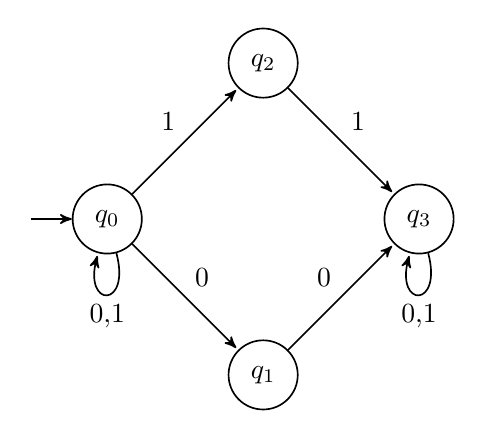
\begin{tikzpicture}[->,>=stealth',shorten >=1pt,auto,node distance=2.8cm,semithick]

        \node[state] (q0)                     {$q_0$};
        \node[state] (q2) [above right of=q0] {$q_2$};
        \node[state] (q1) [below right of=q0] {$q_1$};
        \node[state] (q3) [below right of=q2] {$q_3$};

        \draw[<-] (q0) -- ++(-1cm,0);

        \path (q0) edge [loop below] node {0,1} (q0)
                   edge              node {0}   (q1)
                   edge              node {1}   (q2)
              (q1) edge              node {0}   (q3)
              (q2) edge              node {1}   (q3)
              (q3) edge [loop below] node {0,1} (q3);
        \end{tikzpicture}
    \end{minipage}
    \caption{An NFA.}
    \label{fig:nfa}
\end{figure}

\begin{solution}
    \begin{itemize}
    	\item $I_0 = true$
    	\item $F_3 = true$
    	\item $T_{0, 0, 0} = true, T_{0, 0, 1} = true, T_{0, 1, 0} = true, T_{0, 1, 2} = true$
    	\item $T_{1, 0, 3} = true$
		\item $T_{2, 1, 3} = true$
		\item $T_{3, 0, 3} = true, T_{3, 1, 3} = true$
    \end{itemize}

	Any defined but unlisted propositional variable has the value $false$.
\end{solution}

%% problem ends

\end{document}
